\documentclass[10pt]{article}
\usepackage{icmlko}

\icmlmeta{IP 파운데이션 월드모델}{20}{더 재는 것이 항상 낫지는 않다}{공통 축을 셋으로 늘렸더니 전이가 나빠졌다 --- 축은 개수가 아니라 정의의 정합성이다}

\begin{document}

\twocolumn[
\icmlheader

\begin{abstract}
노트 19는 프로크루스테스 정렬로 라벨 0개 전이를 완성하면서 한계 하나를 적었다 ---
공통 축이 둘이라 적재 행렬이 2$\times$2고 회전에 여유가 없으니 셋으로 늘리라고.
늘렸다. 게임의 미디어 투입이 38\%였던 원인은 퍼블리셔 사전작 부족이었는데,
\textbf{자체 배급 여부}로 메우면 100\%가 된다. 신호도 옳다 --- 자체 배급 218건의
평균 반응이 $-$0.138, 퍼블리셔가 붙은 216건이 $+$0.139다(r=$-$0.139).
\textbf{그런데 전이가 나빠졌다.} 유의 방향이 다섯에서 넷으로 줄고, 평균 차이가
$-$0.0527에서 $-$0.0466으로, 팝업 $\to$ 게임은 p=0.019에서 0.154로 무너졌다.
정렬 기준 축의 부분집합을 전부 돌려 범인을 찾았다 --- \textbf{미디어 투입을 포함한
모든 조합이 나쁘다}(미디어$+$굿즈만 쓰면 유의 방향 1개). 원인은 정의의 불일치다.
세 도메인의 ``미디어 투입''이 서로 다른 것을 잰다 --- 팝업은 기획서의 홍보 계획,
아이돌은 서바이벌과 사전 화제, 게임은 퍼블리셔 실적. 정렬 축에서 빼도 인자 공간을
통해 영향이 남아 축 자체를 되돌렸다. \textbf{공통 축은 개수가 아니라 정의의
정합성으로 고른다.}
\end{abstract}
]

\section{공통 축을 셋으로 늘려 봤다}

노트 19의 한계 절 첫 줄은 이랬다.

\begin{quote}\fontsize{9.2}{11}\selectfont
공통 축이 둘이라 적재 행렬이 2$\times$2다. 회전이 과소결정되지는 않지만 여유도
없다. 공통 축이 셋 이상이면 정렬이 훨씬 안정될 것이다.
\end{quote}

같은 노트의 ``다음'' 첫 항목도 그것이었다 --- 미디어 투입을 게임에서 관측
가능하게 만든다. 게임의 미디어 투입은 퍼블리셔 사전 실적으로 정의했는데 482건 중
185건(38\%)에만 있었다. 표본의 퍼블리셔 대부분이 그 이전 출시작이 없기 때문이다.

메우는 방법이 있었다. \textbf{자체 배급 여부}다. 퍼블리셔가 개발사와 다르다는 것
자체가 홍보 투입의 신호이고, 이것은 100\% 관측된다.

\begin{figure}[t]
\centering
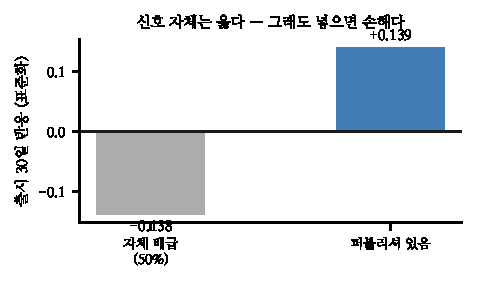
\includegraphics[width=\columnwidth]{figs/selfpub.pdf}
\caption{자체 배급 여부와 출시 30일 반응. 신호의 방향은 옳다.}
\end{figure}

\begin{table}[t]
\centering\tsize
\caption{미디어 투입 후보(n=434).}
\begin{tabular}{lrr}
\toprule
후보 & 커버리지 & 창 라벨과 r \\
\midrule
퍼블리셔 사전 실적 & 38\% & $+$0.338 \\
자체 배급 여부 & \textbf{100\%} & $-$0.139 \\
\bottomrule
\end{tabular}
\end{table}

사전 실적이 있으면 그것을 쓰고 없으면 자체 배급 여부로 대신하도록 결합했다.
커버리지 100\%, 방향도 맞는다. 공통 축이 셋이 됐다.

\section{그런데 나빠졌다}

\begin{figure}[t]
\centering
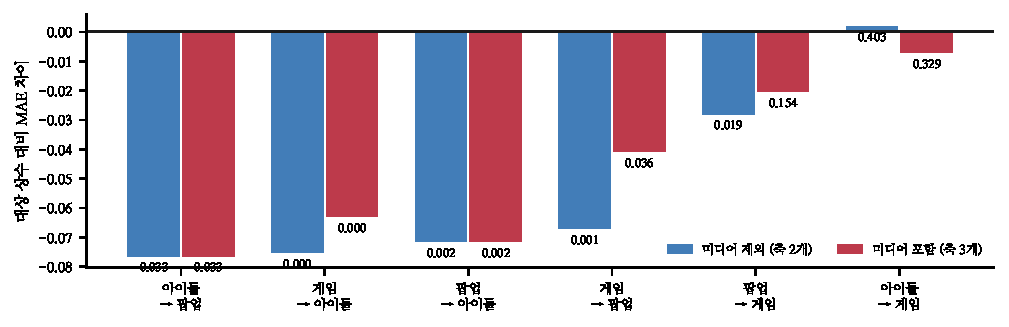
\includegraphics[width=\textwidth]{figs/add.pdf}
\caption{축을 추가하기 전과 후. 여섯 방향 중 넷이 나빠진다.}
\end{figure}

\begin{table}[t]
\centering\tsize
\caption{게임 미디어 투입 추가 전후. 프로크루스테스 정렬, 순열 2,000회.}
\begin{tabular}{lrrrr}
\toprule
& \multicolumn{2}{c}{축 2개} & \multicolumn{2}{c}{축 3개} \\
방향 & 차이 & p & 차이 & p \\
\midrule
팝업 $\to$ 아이돌 & $-$0.0716 & 0.0015 & $-$0.0716 & 0.0015 \\
아이돌 $\to$ 팝업 & $-$0.0765 & 0.0330 & $-$0.0765 & 0.0330 \\
게임 $\to$ 아이돌 & $-$0.0752 & $<$0.0001 & $-$0.0631 & $<$0.0001 \\
게임 $\to$ 팝업 & $-$0.0671 & 0.0005 & $-$0.0409 & 0.0360 \\
팝업 $\to$ 게임 & $-$0.0280 & \textbf{0.0190} & $-$0.0205 & \textbf{0.1540} \\
아이돌 $\to$ 게임 & $+$0.0019 & 0.4025 & $-$0.0072 & 0.3285 \\
\midrule
유의 방향 & \multicolumn{2}{c}{\textbf{5}} & \multicolumn{2}{c}{4} \\
평균 차이 & \multicolumn{2}{c}{\textbf{$-$0.0527}} & \multicolumn{2}{c}{$-$0.0466} \\
\bottomrule
\end{tabular}
\end{table}

관측을 늘렸는데 성능이 떨어졌다. 팝업 $\to$ 게임이 유의성을 잃고, 게임 $\to$ 팝업이
p=0.0005에서 0.036으로 약해졌다. 이득은 아이돌 $\to$ 게임의 부호가 $+$0.0019에서
$-$0.0072로 바뀐 것뿐인데, 둘 다 유의하지 않으므로 실질 이득이 아니다.

\claimx{축을 더 관측 가능하게 만드는 것이 항상 이득은 아니다. 게임의 미디어 투입
커버리지를 38\%에서 100\%로 올리자 유의 전이 방향이 다섯에서 넷으로, 평균 차이가
$-$0.0527에서 $-$0.0466으로 나빠졌다.}{같은 축을 세 도메인에서 같은 방식으로
정의한 뒤 추가했을 때도 나빠지면, 문제는 정의가 아니라 축의 개수 자체다.}

\section{범인을 찾았다}

정렬 기준으로 쓸 축의 부분집합을 전부 돌렸다.

\begin{figure}[t]
\centering
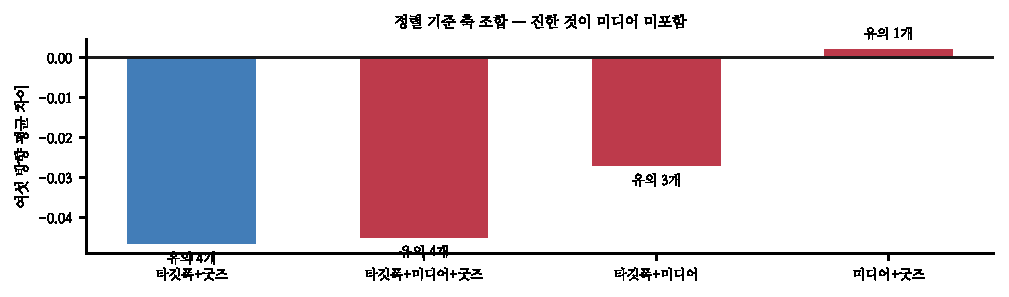
\includegraphics[width=\textwidth]{figs/subset.pdf}
\caption{정렬 기준 축 조합별 성적. 미디어 투입이 들어가면 나빠진다.}
\end{figure}

\begin{table}[t]
\centering\tsize
\caption{정렬 기준 축 조합(순열 2,000회).}
\begin{tabular}{lrr}
\toprule
조합 & 유의 방향 & 평균 차이 \\
\midrule
\textbf{타깃 폭 $+$ 굿즈 규모} & \textbf{4} & \textbf{$-$0.0466} \\
타깃 폭 $+$ 미디어 $+$ 굿즈 & 4 & $-$0.0450 \\
타깃 폭 $+$ 미디어 & 3 & $-$0.0271 \\
미디어 $+$ 굿즈 & 1 & $+$0.0021 \\
\bottomrule
\end{tabular}
\end{table}

미디어 투입이 들어간 조합이 전부 나쁘다. 미디어와 굿즈만으로 정렬하면 유의 방향이
하나로 무너지고 평균 차이가 양수가 된다.

\paragraph{정렬 축에서 빼도 소용없다}
미디어를 정렬 기준에서 빼도 여전히 축 2개 때보다 나쁘다(위 표에서 타깃 폭 $+$ 굿즈
규모 조합이 $-$0.0466인데, 게임에서 미디어 축 자체를 비우면 $-$0.0527이다).
정렬 기준이 아니어도 그 축이 게임의 \emph{인자 공간}에 들어가기 때문이다.
주성분은 관측된 축 전부의 상관 구조에서 나온다.

그래서 축 자체를 되돌렸다. 값은 기록해 두되 마스크를 0으로 되돌려 인자 공간에서
뺐다.

\section{왜 미디어 투입만 이런가}

세 도메인의 ``미디어 투입''이 서로 다른 것을 잰다.

\begin{table}[t]
\centering\tsize
\caption{도메인별 미디어 투입의 정의.}
\begin{tabular}{ll}
\toprule
도메인 & 측정 방법 \\
\midrule
팝업 & 기획서의 홍보 계획을 사람이 0--4로 매김 \\
아이돌 & 서바이벌 출신 $+$ 데뷔 전 화제 $+$ 소속사 실적 \\
게임 & 퍼블리셔 사전 실적 $+$ 자체 배급 여부 \\
\bottomrule
\end{tabular}
\end{table}

팝업은 \emph{계획된 투입}을, 아이돌은 \emph{사전 노출의 결과}를, 게임은
\emph{배급 구조}를 잰다. 이름만 같고 물리량이 다르다.

타깃 폭과 굿즈 규모는 그렇지 않다. 타깃 폭은 세 도메인 모두 ``몇 명에게 닿을 수
있게 만들었나''를 재고(대상 연령대 폭 / 그룹 구성과 대중 노출 / 지원 언어와
플랫폼 수), 굿즈 규모는 ``닿으면 무엇을 얻나''를 잰다(굿즈 종류 / 앨범 버전 /
Steam 기능). 측정 도구는 달라도 재는 것이 같다.

\claimx{공통 축은 개수가 아니라 정의의 정합성으로 고른다. 이름이 같아도 도메인마다
다른 물리량을 재면 인자 공간을 왜곡한다.}{미디어 투입을 세 도메인에서 같은
물리량으로 --- 예컨대 개시 시점 이전 90일간의 언론 노출 건수로 --- 통일해 다시
넣었을 때 전이가 개선되면, 축은 옳고 측정만 어긋났던 것이다.}

이것은 노트 1이 라벨에 대해 말한 것을 축에 대해 되풀이한다. 거기서는 주최자 발표와
게이트 계수가 한 컬럼에 섞여 2.75배 벌어져 있었다. 여기서는 세 가지 다른 측정이
한 축 이름에 섞여 있다. \textbf{이름이 같다고 같은 것이 아니다} --- 라벨에서도,
축에서도.

\section{그래서 노트 19의 권고를 수정한다}

노트 19는 ``공통 축이 셋 이상이면 정렬이 훨씬 안정될 것''이라고 적었다. 절반만
맞다. 정확히는 이렇다.

\begin{quote}\fontsize{9.5}{11.5}\selectfont
공통 축을 늘리면 정렬이 안정된다 --- \textbf{단, 늘리는 축이 세 도메인에서 같은
물리량을 잴 때만.} 정의가 어긋난 축은 늘릴수록 해롭다.
\end{quote}

실행 순서도 바뀐다. 새 축을 공통 축에 넣기 전에 커버리지가 아니라 \emph{정의의
정합성}을 먼저 확인해야 한다. 커버리지는 쉬운 문제이고 정합성은 어려운 문제인데,
쉬운 쪽부터 손대면 이번처럼 된다.

\section{한계}

\begin{itemize}[leftmargin=1.1em,itemsep=0.15em]
\item 정의 불일치가 원인이라는 것은 진단이지 검정이 아니다. 세 도메인의 미디어
      투입을 같은 물리량으로 통일해 재확인해야 한다.
\item 부분집합 검정은 조합 넷뿐이다. 공통 축 후보가 늘면 다중비교가 문제가 된다.
\item 자체 배급 여부의 상관이 $-$0.139로 약하다. 더 강한 신호였다면 정의 불일치를
      이겨냈을 수도 있다.
\item 되돌린 결정은 이 표본에서의 판단이다. 표본이 커지면 뒤집힐 수 있다.
\end{itemize}

\section{다음}

\begin{enumerate}[leftmargin=1.3em,itemsep=0.15em]
\item 미디어 투입을 세 도메인에서 같은 물리량으로 재정의 --- 개시 이전 일정 기간의
      언론 노출 건수처럼 도메인 독립적인 정의.
\item 나머지 축(매장 노출도, 입장 허들)도 정의 정합성 관점에서 재검토.
\item 네 번째 도메인 --- 정합성 원칙이 도메인이 늘어도 유지되는지.
\item 절대량 복원 --- 노트 19가 남긴 과제.
\end{enumerate}

\vspace{0.6em}
\hrule height 0.3pt
\vspace{0.5em}
{\footnotesize
\textbf{참고문헌}\\[0.3em]
Schönemann, P. H. (1966). A generalized solution of the orthogonal Procrustes
problem. \emph{Psychometrika}, 31(1), 1--10.\\[0.15em]
Meredith, W. (1993). Measurement invariance, factor analysis and factorial
invariance. \emph{Psychometrika}, 58(4), 525--543.\\[0.15em]
Guyon, I., Elisseeff, A. (2003). An introduction to variable and feature selection.
\emph{JMLR}, 3, 1157--1182.\\[0.15em]
Ben-David, S. et al. (2010). A theory of learning from different domains.
\emph{Machine Learning}, 79(1--2), 151--175.
}

\end{document}
